\section{Задача 1.27}
\subsection{Задание:}
Не вычисляя определитель
$
	\begin{vmatrix}
		2 & 1 & 7 & 8 & 1 \\
		3 & 9 & 7 & 7 & 4 \\
		6 & 5 & 3 & 4 & 3 \\
		8 & 0 & 4 & 9 & 5 \\
		7 & 2 & 9 & 1 & 9 \\
	\end{vmatrix}
$
доказать что он делится нацело на 947.
\subsection{Решение:}
По свойству определителя к любомоу столбцу можно прибавить линейную комбинацию других, и определитель не изменится.
Прибавим к последнему столбцу линейную комбинацию других:
\\
$
	\tilde a_{\bullet 5} =
	10000 \cdot a_{\bullet 1} +
	1000  \cdot a_{\bullet 2} +
	100   \cdot a_{\bullet 3} +
	10    \cdot a_{\bullet 4}
	+ a_{\bullet 5}
$
\\
Тогда определитель принимает вид:
\\[1em]
$
	\begin{vmatrix}
		2 & 1 & 7 & 8 & 21781 \\
		3 & 9 & 7 & 7 & 39774 \\
		6 & 5 & 3 & 4 & 65343 \\
		8 & 0 & 4 & 9 & 80495 \\
		7 & 2 & 9 & 1 & 72919 \\
	\end{vmatrix}
	=
	947 \cdot
	\begin{vmatrix}
		2 & 1 & 7 & 8 & 23 \\
		3 & 9 & 7 & 7 & 42 \\
		6 & 5 & 3 & 4 & 69 \\
		8 & 0 & 4 & 9 & 85 \\
		7 & 2 & 9 & 1 & 77 \\
	\end{vmatrix}
$
\\[1em]
Значит определитель делится нацело на 947
\subsection{Компьютерная проверка в среде Wolfram Mathematica:}
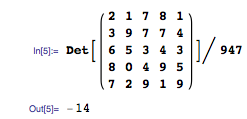
\includegraphics[scale=0.6]{task/1_27/screen1.png}
\subsection{Вывод:}
Компьютерная проверка показала что определитель действительно делится нацело на 947.
